\documentclass[oneside, twocolumn, 9pt, english]{extbook}
\usepackage{supertabular}

\usepackage{../../HPpack}
\usepackage{float}

\begin{document}

\begin{titlepage}

    \centering
    \vfill
    {\bfseries
        {\HP \fontsize{40}{35}\selectfont A Guide to Diagon Alley}
    }    
    \vfill
    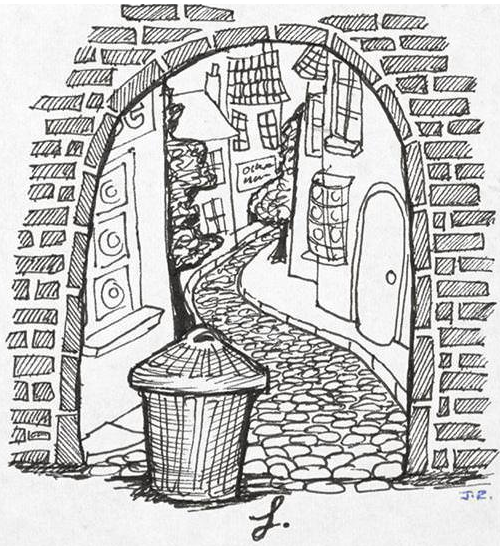
\includegraphics[scale = 0.6]{../../Images/alley} % also works with logo.pdf
    \vfill
    {\HP \fontsize{30}{24} \selectfont  Harry Potter \\\&\\ The Role Playing Game}
    \normalsize
    \vfill
    {\HP \fontsize{22}{0} \selectfont Version 1.0 \hfill Jack Fraser}
\end{titlepage}



	\renewcommand\arraystretch{1.5}
\newcommand\basicPerson[2]
{
	\textbf{\textit{#1}}
	
	#2

}

\newcommand\shop[7]
{
	\subsection{#1 (\it #4)}
	
	\begin{supertabular}{@{} r p{6.5  cm} @{}}
		\bf Location:	&	#2
		\\
		\bf Exterior: &		#5
		\\
		\bf Interior:	&	#6
		\\
		\bf Proprietor:	&	#3
		\\
		\bf Inventory:	&	\parbox[t]{6.5cm}{#7}
		\\
	\end{supertabular}
	~
	\\
}

\setlength\parindent{3pt}
%%ShopBegin
\shop{Daily Prophet HQ}{Diagon Alley}{\basicPerson{Barnabus Cuffe}{The editor\minus{}in\minus{}chief of the Daily Prophet for several decades\comma{} Barnabus Cuffe is an affable gentleman – always seen wearing an impeccable suit and tie underneath a formal wizarding gown. 

His affable demeanor is\comma{} however\comma{} mostly for show and beneath the surface he is a man consumed with the need to accumulate and gather power and influence. He will let nothing (let alone the truth) get in the way of his media empire.} }{Newspaper Printers}{An unassuming building\comma{} without a formal shopfront. 

The only indicators that this is anything other than a residential house is a formal plaque next to the door\comma{} and a dispenser for the Daily Prophet on the street outside.}{The interior is significantly larger than the exterior\comma{} and houses a full magical printing press\comma{} as well as several offices for the prominent journalists. 

The office of the editor is on the second level\comma{} but with a large window capable of overseeing the entire operation.}{Daily Prophet (\knut{8})}

\shop{Eeylops Owl Emporium}{Diagon Alley}{\basicPerson{Frank Blumenthal}{A dour faced man\comma{} who seems not to care for humans whatsoever. Where possible\comma{} he uses a single word to answer a question\comma{} before returning to his owls. 

He only ever cracks a smile when talking about his birds\comma{} which are his whole world. He will refuse to sell an owl if he believes it will be maltreated.} }{Owls}{A huge number of vertical poles stand outside this shop. During daytime\comma{} a multitude of different colour owls occupy them\comma{} cooing and hooting to one another.}{Inside\comma{} the ceiling reaches all the way to the rafters\comma{} creating a very tall (if narrow) space for the owls to fly. Birdcages line the wall\comma{} though the owls themselves seem to roost in special nooks in the walls above headheight.}{A pet owl costs \galleon{1}\comma{} though some of the finer species cost significantly more.}

\shop{Florean Fortescue\apos{}s Ice Cream Parlour}{Diagon Alley}{\basicPerson{Sylvian Fortescue}{The twin brother of the eponymous original proprietor\comma{} Sylvian is an elderly man in his late 90s: balding and with a hooked nose. 

Though elderly in appearance\comma{} he harbours a twinkle in his eye and a spring in his step. A Wonka\minus{}esque pioneer of flavours\comma{} he seems much younger than his advanced years.} }{Ice cream parlour}{A handful of chairs and small tables\comma{} with sunshades\comma{} all a light duck\minus{}egg blue sit outside the storefront\comma{} which (on sunny days) is fully opened to expose the interior to the outside world.}{More chairs and tables are inside the brightly lit interior\comma{} along with a front desk harbouring thousand of flavours of icecream – a multicoloured medly of flavour and sweetness.}{Icecream costs \knut{5} a scoop. 

If you can imagine a flavour\comma{} they have it\comma{} no matter how odd.}

\shop{Flourish \& Blotts}{Diagon Alley}{\basicPerson{Sam Garret}{A severe looking woman with small glasses – your stereotypical high school librarian. 

Though fierce looking\comma{} she takes delight in helping people find the books they need.} }{Books}{A well kept storefront\comma{} with a clean window that allows one to see the bookshelves inside. 

A number of placards out front advertise new arrivals and special offers.}{A central desk is surrounded by hundreds\comma{} thousands of books\comma{} stuffed into bookshelves which line every wall. There us a set of stairs up to another level (with yet more books)\comma{} and several small stepladders float up to customers to help them reach high shelves.}{~\\ There is a link to this inventory at blottsBooks}

\shop{Gringotts Bank}{Diagon Alley}{\basicPerson{Grp’tar}{An aging goblin\comma{} who serves as the primary point of contact for new arrivals\comma{} before directing them to a teller or into the vaults. 

His eyes hold suspicion for everyone\comma{} and he has a distrustful\comma{} dismissive air.} }{Bank}{An enourmous marble clad bulding. A set of marble steps lead visitors up into a giant pillared rotunda with a sky\minus{}blue roof.}{The vast entryway opens up into a large hall\comma{} lined with goblin tellers stacking and counting piles of gold and jewels\comma{} or seeing to customers. 

The proprietor sits on a raised dias in the centre of the hallway. Behind him in a secured area is the entrance to the lower vaults.}{N/A}

\shop{Leaky Cauldron}{Diagon Alley}{\basicPerson{Hannah Abbot}{A blonde lady in her early forties\comma{} with a smiling face and kind eyes. 

Though mostly an unassuming landlady\comma{} under the surface is a trained battlemage – as a member of the DA she faced Voldemort and his Death Eaters. She is currently married to Neville Longbottom.} }{Pub \& Inn}{An old fashioned inn\comma{} above the dorr is mounted a hanging caldron\comma{} perpetually pouring a purple fluid out of it.}{Surprisingly modern\comma{} the wood\minus{}panelled bar area is clean and the smell of cooking food pervades. 

There are several private parlours behind the bar area.}{Soup of the day (\knut{10} )

Hearty Meal (\sickle{4} ) 

Butterbeer (\sickle{2} )

Fire Whiskey (\sickle{2} )}

\shop{Madam Malkin\apos{}s Robes for All Occasions}{Diagon Alley}{\basicPerson{Madam Malkin}{An effortlessly beautiful half\minus{}veela\comma{} everything she does is suffused with elegance and grace. 

She treats every customer as if they were the centre of her entire world\comma{} her warm words layered with kindness and compliments.} }{Clothing}{A simple\comma{} yet stylish storefront. The wooden panelling is freshly painted black\comma{} and shines in sunlight. 

The display window showcases three mannequins in the finest outfits for witches and wizards. 

The sign above the door simply reads {\it MM} in a fancy font.}{Clothing racks towards the front of the store hold numerous robes and outfits of different types. 

Towards the back of the store is an open area where customers go to get measured for custom orders.}{~\\ There is a link to this inventory at malkinList}

\shop{Magical Menagerie}{Diagon Alley}{\basicPerson{Tom Cove}{A short\comma{} squat and unusually ugly man\comma{} with a mess of black hair and lopsided and mishapen features. 

What he lacks in good looks\comma{} he makes up for in charm and personality. A natural salesman and a people person\comma{} he drives a hard bargain.} }{Pets}{The front window of the shop has been converted into a display containing a Murtlap burrow\comma{} such that you can see the underground structure pressed between the glass plates}{The interior contains rows upon rows of cages and tanks of various sizes\comma{} some containing entire ecosystems inside them.}{~\\ There is a link to this inventory at petList}

\shop{Ollivander’s}{Diagon Alley}{\basicPerson{Jenna Ollivander}{A young woman in her early thirties\comma{} though with a shock of grey\minus{}white hair which sticks out at odd angles. 

She is excitable\comma{} and has a nervous energy as she darts around her shop\comma{} jumping and skipping as she goes. Though the boxes have no labels\comma{} she seems to be able to find whatever she is looking for.} }{Magical wands}{A tall\comma{} narrow building barely wide enough to fit two people abrest. 

The green sign above the door has the name written in large golden letters.}{Narrow and cramped\comma{} with every wall covered in row upon row of wandboxes. The light is suffused with  magical energy.}{Ollivander\apos{}s has all normal wands for sale at \galleon{5} each. 

To buy a wand\comma{} you must roll on the wand table.}

\shop{Quality Quidditch Supplies}{Diagon Alley}{\basicPerson{Seamus Finnigan}{An irish gentleman\comma{} in his mid\minus{}forties and the lack of hair to prove it. 

Deeply passionate about quidditch\comma{} he will talk for hours to customers about their purchases\comma{} and ensure they have exactly what they need.} }{Brooms}{A large window display prominently shows the latest model of broomstick\comma{} as well as mannequins wearing the uniforms for some of the larger quidditch teams.}{Wall\minus{}mounted racks hold many different broomsticks\comma{} and a number of snitches buzz around in the air buffeting into customers.}{~\\ There is a link to this inventory at qqSupplies}

\shop{Rosa Lee Teashop}{Diagon Alley}{\basicPerson{Rosa Lee}{A short\comma{} plump lady dressed all in purple – including dyed purple hair. 

Homely and kind\comma{} she takes joy in feeding people\comma{} and will often slip an extra slice onto the plates of those she thinks are a bit malnourished.} }{Food \& Drink}{A quaint little teashop\comma{} with a purple exterior. A large window opens onto the kitchen\minus{}area\comma{} showing a set of enchanted kitchen tools preparing fresh cakes.}{Inside is an explosion of colour – paisly tablecloths and tartan teapots\comma{} with polka dot chairs. 

Nothing matches\comma{} and everything is garish – and yet it somehow manages to avoid crossing the line into tacky.}{Afternoon tea (\sickle{5})

Slice of cake (\knut{15} )}

\shop{Slug \& Jiggers Apothecary}{Diagon Alley}{\basicPerson{Jemima Poffley}{A young woman in her mid\minus{}twenties\comma{} with closely cropped hair and a large pair of glasses. 

She has a nervous stutter\comma{} and seem unsure of herself – until she starts talking about alchemical ingredients\comma{} at which point she becomes filled with confidence.} }{Alchemy}{The outside of the shop is almost entiely obscured by a thick rolling fog that seems to be coming from a top floor window. Every few minutes\comma{} there’s a loud {\it crack} sound\comma{} and the colour of the smoke changes – usually accompanied by some choice curses.}{Inside the air is clean and fresh\comma{} and smells of fresh picked grass and other herbs. 

Various alchemical supplies line the walls in neat little jars\comma{} meticulously labelled. 

The centre of the room has some larger merchandise – cauldrons and alchemical filters.}{~\\ There is a link to this inventory at alchemyList}

\shop{Sugarplum Sweetshop}{Diagon Alley}{\basicPerson{Jo King}{An elderly man\comma{} with bright blue hair\comma{} and only a single tooth. 

A talks with a lisp\comma{} but is full of vim and vigour. He has a special (non creepy) fondness for children\comma{} and delights in finding them new sweets that they have  never experienced before.} }{Sweets}{The window is stacked full of displays showcasing sweets and treats – from old favourites to the newest imports. 

A goblin employee outside stands with a tray of free samples\comma{} attempting (though mostly failing) to entice people inside.}{An amazingly stocked\comma{} traditional sweet shop. Enormous jars filled with goodies line every wall\comma{} and children dart around filling up paper bags with their favourite sweets.}{Acid Pops (\knut{12})

Bertie Botts Every Flavour Beans (\knut{5})

Chocolate Frogs (pack of 3 \minus{} \sickle{1})

Fizzing Whisbees (\sickle{1})

Liquorice Wands (\knut{15})}

\shop{The Junk Shop}{Diagon Alley}{\basicPerson{Lomp}{Unmistakeably a man with significant amounts of giant blood in him\comma{} Lomp stands a full 7 feet tall\comma{} and seems almost as wide. 

Matted blond hair falls to his mid back\comma{} and his outfit is an insane medley of colours and styles. His fingers have an assortment of rings and other decorations (most of which are hideous and obviously made of actual rubbish). 

He is very possessive of the stuff in his shop\comma{} and gets very defensive when it is insulted as useless.} }{Various}{The exterior of this shop is almost non\minus{}existent – it is simply a door wedged inside a great mound of crates stacked outside the font of the shop\comma{} obscuring everything else about the bulding and spilling out onto the street.}{A dark\comma{} fusty and cramped interior\comma{} the room is filled with rows upon rows of shelves covered in what is almost entirely rubbish. 

The stuff does not smell\comma{} but it comprises of broken pottery and dented metal plates\comma{}  Threadbare blankets and two\minus{}legged chairs.}{~\\ There is a link to this inventory at junkList}

\shop{Weasley\apos{}s Wizard Wheezes}{Diagon Alley}{\basicPerson{George Weasley}{A one\minus{}eared\comma{} red\minus{}haired jokester\comma{} who spends most of his time playing pranks on his customers\comma{} rather than trying to sell them anything. 

Unusually\comma{} however\comma{} this business model has turned out to be an incredible success\comma{} and George and his brother Ron have turned this into a successful business.} }{Prank shop}{A prominent shop\comma{} right on the street corner\comma{} made even more noticeable by the large weasley\minus{}esque statue mounted atop the frontage. This statue is known to make rude gestures and blow raspberries at passers by.}{A wide open shop floor\comma{} with a cacophany of noise as George prances round\comma{} demonstrating his wares. 

Small alcoves are found at the back where the pricier items are held\comma{} and in the front are vast vats of their best selling items.}{~\\ There is a link to this inventory at weasleyList}

\shop{Wiseacre\apos{}s Wizarding Equipment}{Diagon Alley}{\basicPerson{}{} }{}{}{}{}

\shop{Borgin \& Burke\apos{}s}{Nockturn Alley}{\basicPerson{}{} }{}{}{}{}

\shop{Cobb and Webb\apos{}s}{Nockturn Alley}{\basicPerson{}{} }{}{}{}{}

\shop{Mulpepper\apos{}s Apothecary}{Nockturn Alley}{\basicPerson{}{} }{}{}{}{}

\shop{Shyverwretch\apos{}s Venoms and Poisons}{Nockturn Alley}{\basicPerson{}{} }{}{}{}{}

\shop{The Coffin House}{Nockturn Alley}{\basicPerson{}{} }{}{}{}{}

\shop{White Wyvern}{Nockturn Alley}{\basicPerson{}{} }{}{}{}{}

\shop{Warcasters}{Venter Alley}{\basicPerson{}{} }{}{}{}{}

\shop{Simon\apos{}s Simple Shields}{Venter Alley}{\basicPerson{}{} }{}{}{}{}

\shop{Ministry Portal}{Venter Alley}{\basicPerson{}{} }{}{}{}{}


%%ShopEnd


\end{document}
